% Options for packages loaded elsewhere
\PassOptionsToPackage{unicode}{hyperref}
\PassOptionsToPackage{hyphens}{url}
\PassOptionsToPackage{dvipsnames,svgnames,x11names}{xcolor}
%
\documentclass[
  12pt,
  a4paper,
  DIV=11,
  numbers=noendperiod]{scrartcl}

\usepackage{amsmath,amssymb}
\usepackage{iftex}
\ifPDFTeX
  \usepackage[T1]{fontenc}
  \usepackage[utf8]{inputenc}
  \usepackage{textcomp} % provide euro and other symbols
\else % if luatex or xetex
  \usepackage{unicode-math}
  \defaultfontfeatures{Scale=MatchLowercase}
  \defaultfontfeatures[\rmfamily]{Ligatures=TeX,Scale=1}
\fi
\usepackage{lmodern}
\ifPDFTeX\else  
    % xetex/luatex font selection
\fi
% Use upquote if available, for straight quotes in verbatim environments
\IfFileExists{upquote.sty}{\usepackage{upquote}}{}
\IfFileExists{microtype.sty}{% use microtype if available
  \usepackage[]{microtype}
  \UseMicrotypeSet[protrusion]{basicmath} % disable protrusion for tt fonts
}{}
\makeatletter
\@ifundefined{KOMAClassName}{% if non-KOMA class
  \IfFileExists{parskip.sty}{%
    \usepackage{parskip}
  }{% else
    \setlength{\parindent}{0pt}
    \setlength{\parskip}{6pt plus 2pt minus 1pt}}
}{% if KOMA class
  \KOMAoptions{parskip=half}}
\makeatother
\usepackage{xcolor}
\usepackage[top=20mm,left=20mm,heightrounded]{geometry}
\setlength{\emergencystretch}{3em} % prevent overfull lines
\setcounter{secnumdepth}{-\maxdimen} % remove section numbering
% Make \paragraph and \subparagraph free-standing
\ifx\paragraph\undefined\else
  \let\oldparagraph\paragraph
  \renewcommand{\paragraph}[1]{\oldparagraph{#1}\mbox{}}
\fi
\ifx\subparagraph\undefined\else
  \let\oldsubparagraph\subparagraph
  \renewcommand{\subparagraph}[1]{\oldsubparagraph{#1}\mbox{}}
\fi


\providecommand{\tightlist}{%
  \setlength{\itemsep}{0pt}\setlength{\parskip}{0pt}}\usepackage{longtable,booktabs,array}
\usepackage{calc} % for calculating minipage widths
% Correct order of tables after \paragraph or \subparagraph
\usepackage{etoolbox}
\makeatletter
\patchcmd\longtable{\par}{\if@noskipsec\mbox{}\fi\par}{}{}
\makeatother
% Allow footnotes in longtable head/foot
\IfFileExists{footnotehyper.sty}{\usepackage{footnotehyper}}{\usepackage{footnote}}
\makesavenoteenv{longtable}
\usepackage{graphicx}
\makeatletter
\def\maxwidth{\ifdim\Gin@nat@width>\linewidth\linewidth\else\Gin@nat@width\fi}
\def\maxheight{\ifdim\Gin@nat@height>\textheight\textheight\else\Gin@nat@height\fi}
\makeatother
% Scale images if necessary, so that they will not overflow the page
% margins by default, and it is still possible to overwrite the defaults
% using explicit options in \includegraphics[width, height, ...]{}
\setkeys{Gin}{width=\maxwidth,height=\maxheight,keepaspectratio}
% Set default figure placement to htbp
\makeatletter
\def\fps@figure{htbp}
\makeatother
% definitions for citeproc citations
\NewDocumentCommand\citeproctext{}{}
\NewDocumentCommand\citeproc{mm}{%
  \begingroup\def\citeproctext{#2}\cite{#1}\endgroup}
\makeatletter
 % allow citations to break across lines
 \let\@cite@ofmt\@firstofone
 % avoid brackets around text for \cite:
 \def\@biblabel#1{}
 \def\@cite#1#2{{#1\if@tempswa , #2\fi}}
\makeatother
\newlength{\cslhangindent}
\setlength{\cslhangindent}{1.5em}
\newlength{\csllabelwidth}
\setlength{\csllabelwidth}{3em}
\newenvironment{CSLReferences}[2] % #1 hanging-indent, #2 entry-spacing
 {\begin{list}{}{%
  \setlength{\itemindent}{0pt}
  \setlength{\leftmargin}{0pt}
  \setlength{\parsep}{0pt}
  % turn on hanging indent if param 1 is 1
  \ifodd #1
   \setlength{\leftmargin}{\cslhangindent}
   \setlength{\itemindent}{-1\cslhangindent}
  \fi
  % set entry spacing
  \setlength{\itemsep}{#2\baselineskip}}}
 {\end{list}}
\usepackage{calc}
\newcommand{\CSLBlock}[1]{\hfill\break\parbox[t]{\linewidth}{\strut\ignorespaces#1\strut}}
\newcommand{\CSLLeftMargin}[1]{\parbox[t]{\csllabelwidth}{\strut#1\strut}}
\newcommand{\CSLRightInline}[1]{\parbox[t]{\linewidth - \csllabelwidth}{\strut#1\strut}}
\newcommand{\CSLIndent}[1]{\hspace{\cslhangindent}#1}

\KOMAoption{captions}{tableheading}
\usepackage{wrapfig}
\usepackage{subcaption}
\usepackage{amsmath}
\usepackage{cancel}
\renewcommand{\maketitle}{}
\usepackage{tikz}
\makeatletter
\@ifpackageloaded{caption}{}{\usepackage{caption}}
\AtBeginDocument{%
\ifdefined\contentsname
  \renewcommand*\contentsname{Table of contents}
\else
  \newcommand\contentsname{Table of contents}
\fi
\ifdefined\listfigurename
  \renewcommand*\listfigurename{Figurliste}
\else
  \newcommand\listfigurename{Figurliste}
\fi
\ifdefined\listtablename
  \renewcommand*\listtablename{Tabelliste}
\else
  \newcommand\listtablename{Tabelliste}
\fi
\ifdefined\figurename
  \renewcommand*\figurename{Figur}
\else
  \newcommand\figurename{Figur}
\fi
\ifdefined\tablename
  \renewcommand*\tablename{Tabell}
\else
  \newcommand\tablename{Tabell}
\fi
}
\@ifpackageloaded{float}{}{\usepackage{float}}
\floatstyle{ruled}
\@ifundefined{c@chapter}{\newfloat{codelisting}{h}{lop}}{\newfloat{codelisting}{h}{lop}[chapter]}
\floatname{codelisting}{Listing}
\newcommand*\listoflistings{\listof{codelisting}{List of Listings}}
\makeatother
\makeatletter
\makeatother
\makeatletter
\@ifpackageloaded{caption}{}{\usepackage{caption}}
\@ifpackageloaded{subcaption}{}{\usepackage{subcaption}}
\makeatother
\ifLuaTeX
  \usepackage{selnolig}  % disable illegal ligatures
\fi
\usepackage{bookmark}

\IfFileExists{xurl.sty}{\usepackage{xurl}}{} % add URL line breaks if available
\urlstyle{same} % disable monospaced font for URLs
\hypersetup{
  colorlinks=true,
  linkcolor={blue},
  filecolor={Maroon},
  citecolor={Blue},
  urlcolor={Blue},
  pdfcreator={LaTeX via pandoc}}

\author{}
\date{}

\begin{document}


\newgeometry{left=0cm, right=0cm, top=0cm, bottom=0cm}
\vspace*{0.5cm} 
\hspace*{1.5cm}
\includegraphics[width=10cm]{UiT_Logo_Bok_Bla_RGB.png} 

\begin{flushleft}
    \vspace*{0.5cm}
    \fontsize{12}{13.2}\selectfont
    \hspace*{2.5cm}Handelshøgskolen ved UiT \\[0.2em]
    \hspace*{2.5cm}{\fontsize{7}{12}\selectfont Fakultet for biovitenskap, fiskeri og økonomi} \\[0.2em]
    \hspace*{2.5cm}\large{\textbf{Utfordring 1}}  \\[0.5em]
    \hspace*{2.5cm}\fontsize{11}{13.2}\selectfont Teoretisk analyse av Solow-modellen \\[0.5em]
    \hspace*{2.5cm}Kandidatnummer: 70, 84, 72 \\[0.5em]
    \hspace*{2.5cm}Sok-2011, Vår 2024 \\[0.5em]
\end{flushleft} 

\begin{tikzpicture}[remember picture, overlay]
    \node[anchor=south west, inner sep=0] at (current page.south west) {
\includegraphics[width=\paperwidth]{forside_bilde.png}};
\end{tikzpicture}


\newgeometry{left=20mm, right=20mm, top=20mm, bottom=20mm}

\newpage
\hypersetup{linkcolor=black}
\renewcommand{\contentsname}{Innholdsfortegnelse}
\renewcommand*{\figureautorefname}{Figur}
\renewcommand*{\tableautorefname}{Tabell}
\tableofcontents
\listoffigures
\newpage

\section{Utfordring 1.1 Solow
grunnmodell}\label{utfordring-1.1-solow-grunnmodell}

Solow-modellen predikerer at nivået på spareraten og
befolkningsvekstraten, er helt sentrale for nivået på produksjonen per
arbeider på lang sikt (steady state).

\subsubsection{Antakelser i solow sin
grunnmodell}\label{antakelser-i-solow-sin-grunnmodell}

Før vi utleder Solow-modellen så må vi ta for oss en del antagelser som
må ligge til grunn for å best mulig og enklest gjøre det sammenlignbart.
Og i forhold til den grunnleggende Solow-modellen så går man ut fra
disse antakelsene:

\begin{enumerate}
\def\labelenumi{\arabic{enumi}.}
\item
  Alle bedrifter produserer et homogent gode.
\item
  Fullkommen konkurranse, som vil si at bedriftene har en profitt på
  kroner 0.
\item
  En har to produksjonsfaktorer, arbeid og kapital, definert ved
  \(Prod(Y)=Kapital(k) \> og \> arbeid(L)\)
\item
  Konstant skalautbytte og avtakende marginal produktivitet, som vil si
  at ved konstant skalautbytte så vil for eksempel en dobling i
  innsatsfaktor(ene) gi en dobling i produksjonen, men siden den også er
  avtagende i marginalproduktiviteten så vil økningen i produksjonen
  være avtagende for hver økning
\item
  Alle i befolkningen (p) er i arbeid. \(L=p\), det tas ikke hensyn til
  de som ikke er i stand til å jobbe, alle regnes under ett.
\item
  Befolkningen vokser med en konstant, eksogent gitt rate (n):
  \(L(t)=L_0 e^{nt}\)
\item
  Spareraten(netto) er eksogent gitt. og er lik for alle. og er en andel
  av den totale inntekten. \(0\leq S\leq 1\)
\item
  Lukket økonomi. som vil si at Import = 0 = Eksport, altså ingen handel
  med utlandet.
\end{enumerate}

\paragraph{Konsekvenser ved
antagelsene.}\label{konsekvenser-ved-antagelsene.}

\begin{enumerate}
\def\labelenumi{\arabic{enumi}.}
\item
  All produksjon blir inntekt. Som er et mål på konsum-muligheten og som
  igjen er et mål på materiell velferd.
\item
  Sparing = Investering. All sparing blir produktivt kapital. Positiv
  nettosparing fører til vekst i kapitalstokken.
\end{enumerate}

\clearpage

\subsubsection{Utledning av steady-state-nivået i grunnleggende
Solow-modell
matematisk}\label{utledning-av-steady-state-nivuxe5et-i-grunnleggende-solow-modell-matematisk}

Vi definerer produksjons-funksjonen hvor produksjonen avhenger av
kapital og arbeid. \(1 >\alpha > 0\)
\[ Y(t) = K(t)^\alpha L(t)^{1-\alpha}\]

Y viser oss BNP der kapital og arbeidskraft er de eneste
produksjonsfaktorene, men på grunn av avtakende grenseproduktivitet vist
med \(\alpha\) og \(1-\alpha\) ,så vil en økt mengde av enten kapital
eller arbeidskraft bidra mindre enn 1:1 til totalproduksjonen.

\fbox{
 \addtolength{\linewidth}{-2\fboxsep}%
 \addtolength{\linewidth}{-2\fboxrule}%
 \begin{minipage}{\linewidth}
  \begin{equation}
    Y(t) = K(t)^\alpha \cdot L(t)^{1-\alpha}
  \end{equation}
  \begin{equation}
    \frac{Y(t)}{L(t)} = \frac{K(t)^\alpha \cdot L(t)^{1-\alpha}}{L(t)}
  \end{equation}
  \begin{equation}
    y(t) = K(t)^\alpha \cdot L(t)^{1-\alpha}\cdot L(t)^{-1}
  \end{equation}
  \begin{equation}
    y(t) = K(t)^\alpha \cdot L(t)^{1-\alpha-1} \rightarrow K(t)^\alpha \cdot L(t)^{-\alpha} \rightarrow \left( \frac{K(t)}{L(t)} \right)^\alpha
  \end{equation}
  \begin{equation}
    y(t) = \left( \frac{K(t)}{L(t)} \right)^\alpha 
  \end{equation}
  \begin{equation}
    y(t) =  k(t)^\alpha
  \end{equation}
 \end{minipage}
}

\(y(t) = k(t)^\alpha\) viser forholdet mellom kapital per arbeider og
produksjon per arbeider. På denne måten kan vi se at det som påvirker
BNP per arbeider er avhengig av hvor mye kapital som er tilgjengelig per
arbeider. For eksempel vil det gi oss en lav BNP, dersom det var 1
traktor for hver 10 arbeider, men dersom det var 1 traktor for hver
arbeider så vil BNP per arbeider være høyere. Samtidig kan vi se at
dersom hver arbeider da hadde 2 traktorer så ville det ikke bidratt like
mye til BNP per arbeider som det den første traktoren gjorde.

Ved å ta logaritmen av begge sider av likning (6) får vi
\[ \ln y(t) = \alpha \cdot \ln k(t)\]

Ved å derivere begge sider med hensyn på \(t\), så får vi
\[ \frac{\frac{\partial}{\partial t} y{\left(t \right)}}{y{\left(t \right)}} = \frac{\alpha \frac{\partial}{\partial t} k{\left(t \right)}}{k{\left(t \right)}} \]

Dette skriver vi så om til
\[ \frac{1}{y(t)} \cdot \frac{\partial y(t)}{\partial t} = \alpha \cdot \frac{1}{k(t)} \cdot \frac{\partial k(t)}{\partial t}\]

Vi blir å skrive
\(\frac{1}{y(t)} \cdot \frac{\partial y(t)}{\partial t}\) som \(g_y(t)\)
og \(\frac{1}{k(t)} \cdot \frac{\partial k(t)}{\partial t}\) som
\(g_k(t)\)

Som da gir oss

\[g_y = \alpha \cdot g_k\]

For å finne vekst i kapital per arbeider, så må vi se på hva vi vet om
\(k(t)\). Antagelse 6 er gitt i ligning 9.

\fbox{
 \addtolength{\linewidth}{-2\fboxsep}%
 \addtolength{\linewidth}{-2\fboxrule}%
 \begin{minipage}{\linewidth}
  \begin{equation}
    k(t) = \frac{K(t)}{L(t)}
  \end{equation}
  \begin{equation}
    \frac{\partial k(t)}{\partial t} = s \cdot y(t)
  \end{equation}
  \begin{equation}
    L(t) = L_0 \cdot e^{n\cdot t} 
  \end{equation}
 \end{minipage}
}

Som vist i ligning 9 så vokser L med en eksogent gitt og konstant rate.

Tar logaritmen av ligning 7 \(\ln(k(t)) = \ln(K((t)) - \ln(L(t))\) og
deriverer.

\[\frac{1}{k(t)} \cdot \frac {\partial k(t)}{\partial t} = \frac{1}{K(t)}- \frac{1}{L(t)} \cdot \frac{\partial L(t)}{\partial t}\]

\[\frac{1}{K(t)} = s \cdot Y(t) \frac{\partial L(t)}{\partial t} = n\]

\[\frac{1}{k(t)} \cdot \frac {\partial k(t)}{\partial t} = \frac{s \cdot Y(t)}{K(t)}- n\]

Deler så for å få det i per arbeider

\[\frac{1}{k(t)} \cdot \frac {\partial k(t)}{\partial t} = s \cdot \frac{\frac{Y(t)}{L(t)}}{\frac{K(t)}{L(t)}} -n\]

\[\frac{1}{k(t)} \cdot \frac {\partial k(t)}{\partial t} = s \cdot \frac{y(t)}{k(t)} - n\]

\[\frac{1}{k(t)} \cdot \frac {\partial k(t)}{\partial t} = s \cdot \frac{k^\alpha}{k} - n\]

deler så inn på k

\[\frac{\partial k}{\partial t} = s \cdot \frac{k^\alpha}{k}-n\]

\[\frac{\partial k}{ \partial t} = s \cdot k^\alpha - n \cdot k \tag{10}\]

Vilkåret for steady-state er da at ligning 10 er lik 0.

\fbox{
 \addtolength{\linewidth}{-2\fboxsep}%
 \addtolength{\linewidth}{-2\fboxrule}%
 \begin{minipage}{\linewidth}
  \begin{equation}
    s \cdot k^{\alpha} - n \cdot k = 0
  \end{equation}
  \begin{equation}
    s \cdot k^{\alpha} = n \cdot k
  \end{equation}
  \begin{equation}
    \frac{s \cdot k^{\alpha}}{n} = k
  \end{equation}
  \begin{equation}
    \frac{s \cdot \cancel{k^{\alpha}}}{n} \cdot \frac{1}{\cancel{k^{\alpha}}} = k \cdot \frac{1}{k^{\alpha}}
  \end{equation}
  \begin{equation}
   \frac{s}{n} = k \cdot \frac{1}{k^\alpha}
  \end{equation}
  \begin{equation}
    \frac{s}{n} = k^{1-\alpha}
  \end{equation}
  \begin{equation}
    \left( \frac{s}{n}\right)^\frac{1}{1-\alpha} = \left(k^{\cancel{1-\alpha}}\right)^{\cancel{\frac{1}{1-\alpha}}}
  \end{equation}
  \begin{equation}
    k^{ss}=\left( \frac{s}{n}\right)^{\frac{1}{1-\alpha}}
  \end{equation}
 \end{minipage}
}

Siden \(y(t)=k^\alpha\) så får vi da
\(y^{ss}=\left(k^{ss}\right)^\alpha\)

\(y^{ss}=\left(\left( \frac{s}{n}\right)^\frac{1}{1-\alpha}\right)^\alpha\)

ganger ut parentesene og får

\[y^{ss}=\left( \frac{s}{n}\right)^\frac{\alpha}{1-\alpha}\]

som viser steady-state nivået for kapital per arbeider, som er punktet
hvor økonomien ikke lenger opplever per arbeider vekst i kapital eller
produksjon. Dette forteller oss at for en gitt kombinasjon av sparerate
og befolknings-vekstrate er det et nivå av kapital per arbeider som
økonomien vil konvergere mot over tid. Å ha 2 traktorer per arbeider vil
være dyrt i drift og vil dermed lede til at det blir mindre kapital per
arbeider som demper produksjonen, det motsatte skjer når det er langt
færre traktorer enn det faktisk trengs, da alle som investerte penger i
traktorer til arbeiderne, ville opplevd en stor avkastning og ville
investert opp til det konvergerings-punktet. En høyere sparerate eller
en lavere befolkningsvekst vil føre til et høyere steady-state nivå av
kapital per arbeider.

\clearpage

\subsection{Likevekt, sparerate og
befolkningsvekst-rate}\label{likevekt-sparerate-og-befolkningsvekst-rate}

\begin{wrapfigure}{r}{0.5\textwidth}
    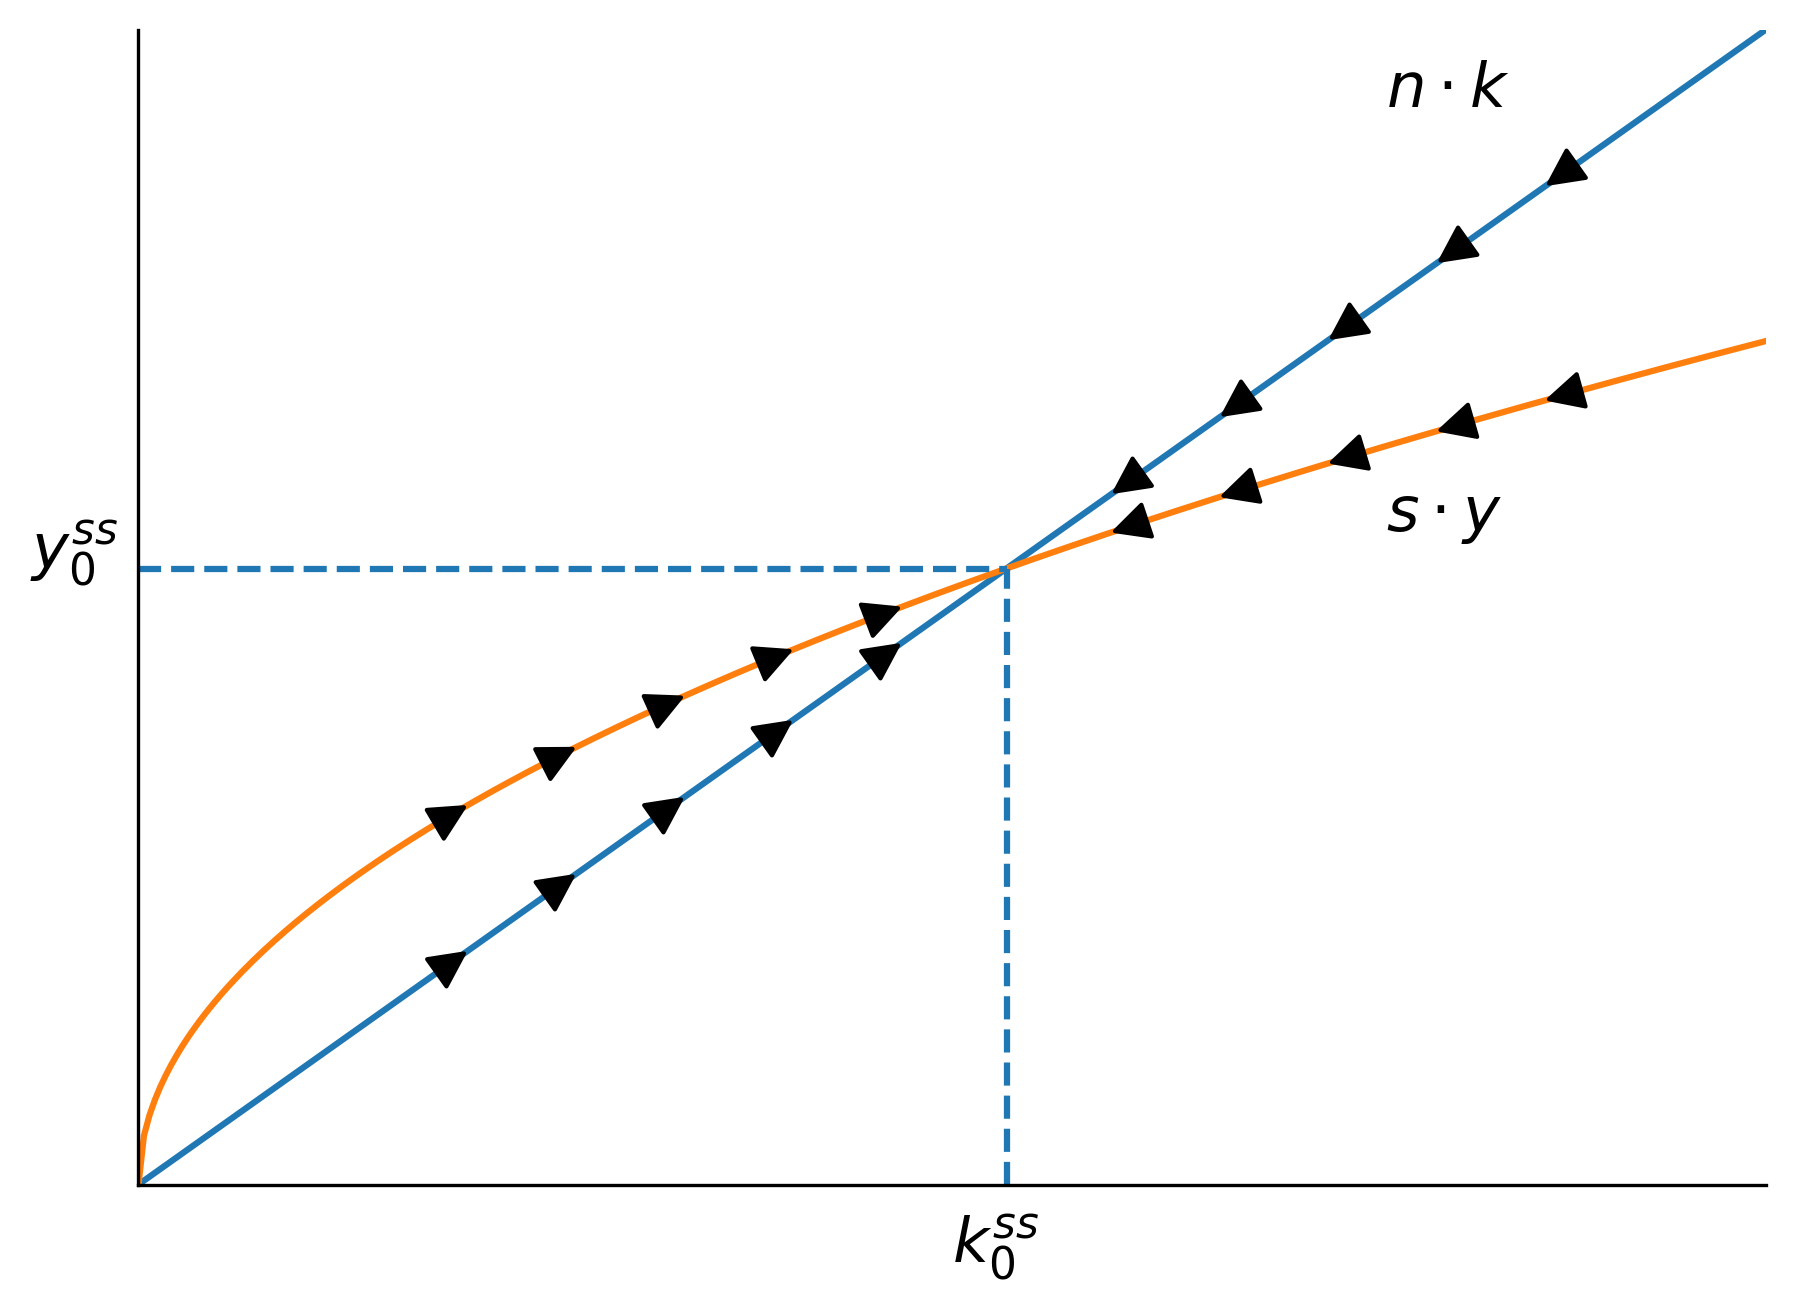
\includegraphics[width=0.48\textwidth]{Likevekt_grunnleggende.png}
  \caption{Likevekt i den grunnleggende Solow-modellen}
  \label{fig:likevekt_grunnleggende}
  \vspace{-12mm}
\end{wrapfigure}

\autoref{fig:likevekt_grunnleggende} viser langsiktig likevekt i den
grunnleggende Solow-modellen. Vist med piler er hva som vil skje dersom
y hadde vært på et annet punkt på s \cdot y linjen. De vil bevege seg
mot steady-state nivået og stabiliseres der. Det er punktet der hvor
nettoinvesteringer er lik de nødvendige investeringer, for å holde
kapital per arbeider konstant.

Så en økning i s vil gi høyere k og y.

\(k^{ss}=\left( \frac{s}{n}\right)^{\frac{1}{1-\alpha}}\)

\(y^{ss}=\left( \frac{s}{n}\right)^\frac{\alpha}{1-\alpha}\)

\begin{figure}[b]
  \centering
  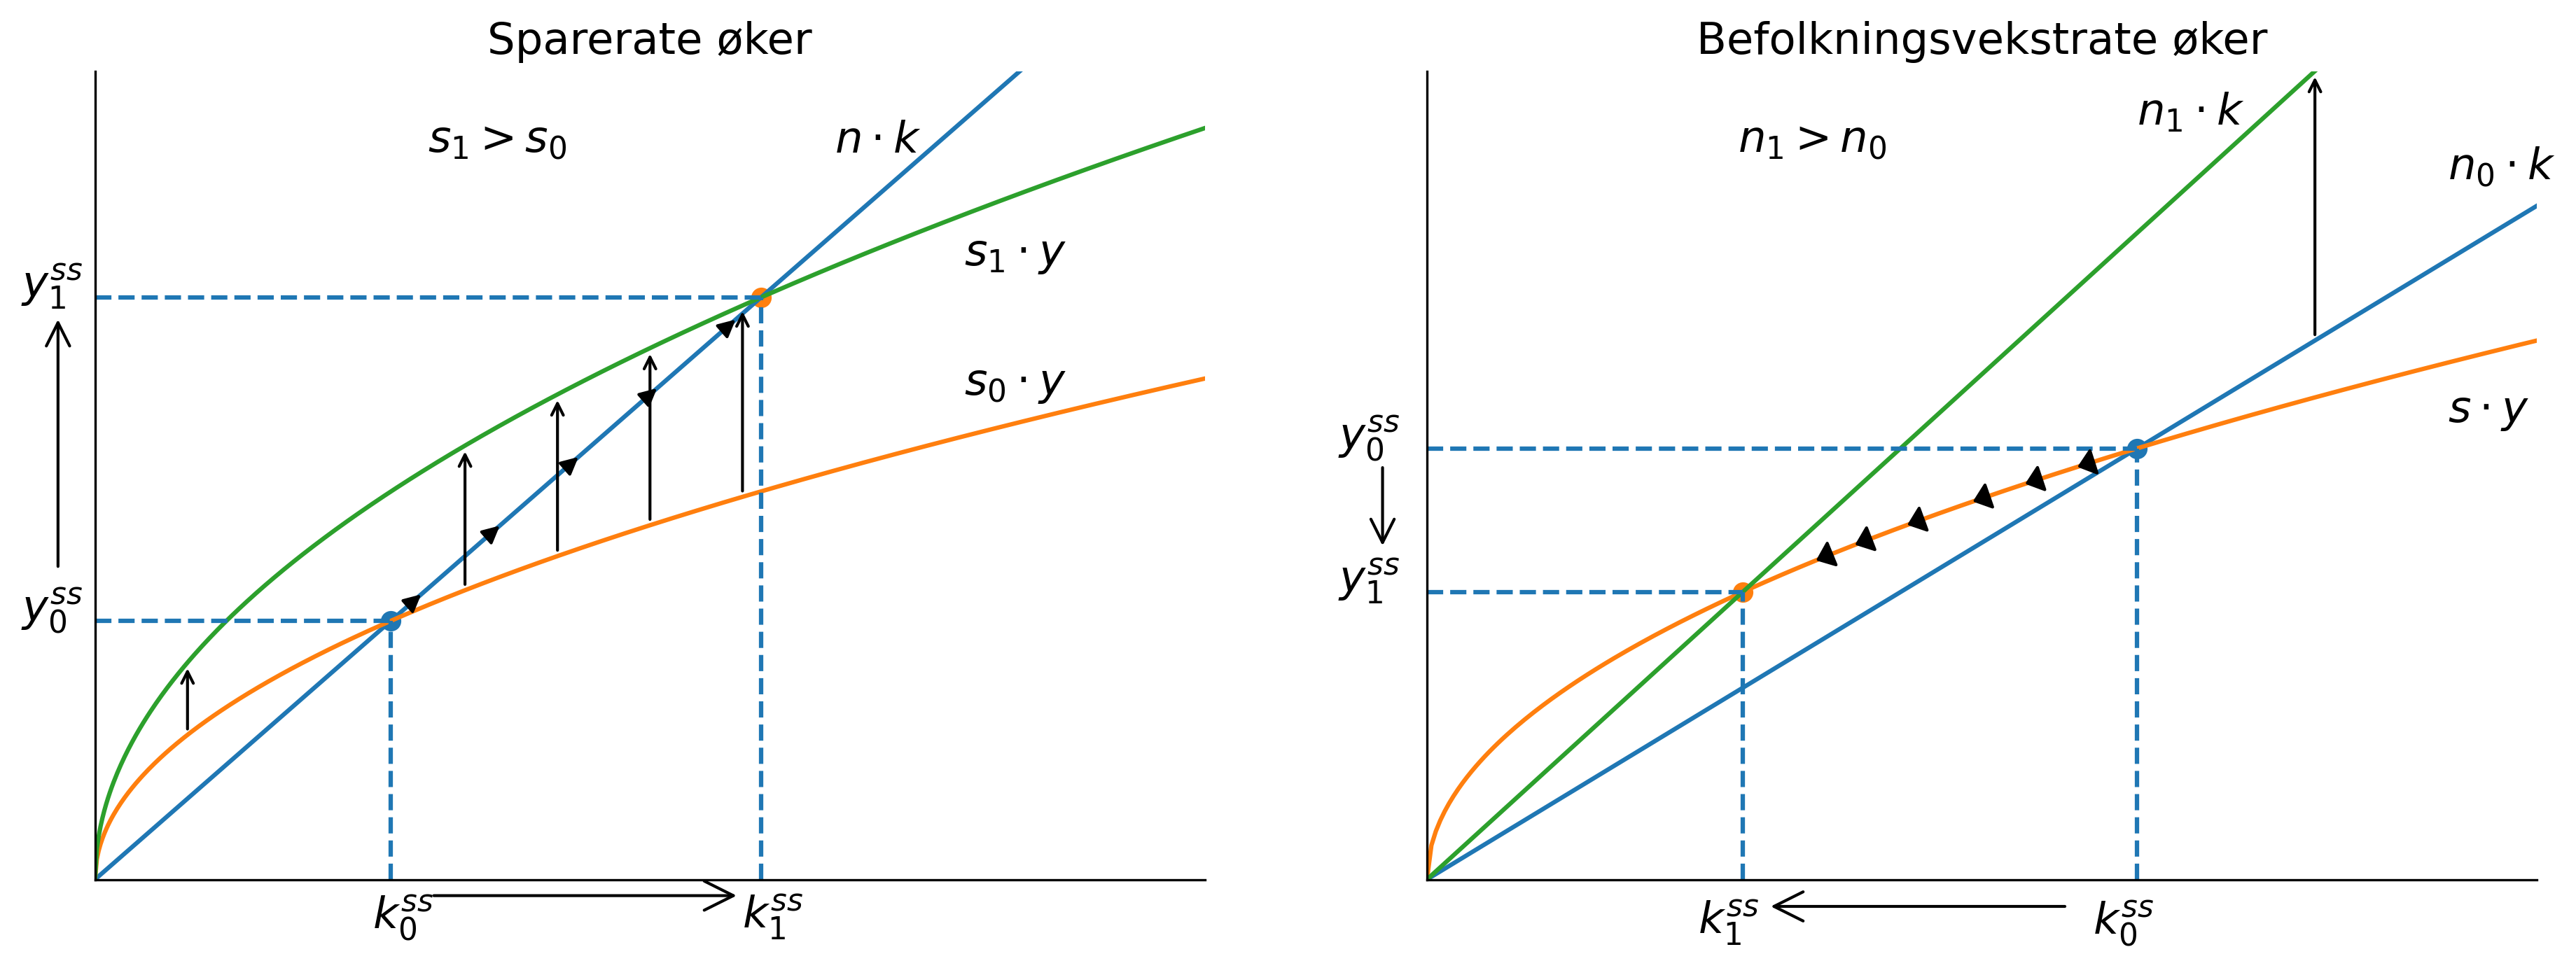
\includegraphics[width=\linewidth]{Figur2og3.png}
  \captionof{figure}{Spareranten endres og befolkningsvekstraten endres}
  \label{fig:fig4}
\end{figure}

\autoref{fig:fig4} viser hva som skjer når spareraten eller
befolknings-vekstraten øker. Økning i spareraten gir et høyere nivå av
\(k^{ss}\) siden mer av hvert års produksjon blir spart og investert i
stedet for konsumert. Dette resulterer i en høyere \(y^{ss}\). Så en
økning i \(s\) vil gi høyere \(k\) og \(y\).

En økning i befolknings-vekstraten reduserer \(k^{ss}\) og \(y^{ss}\)
fordi den samme mengden investeringer nå må fordeles over flere
arbeidere. Hvis befolkningen vokser raskere, så trenges det mer kapital
per arbeider, som gjør at produksjon per arbeider går ned.

\clearpage

\section{Utfordring 1.2
Konvergensteori}\label{utfordring-1.2-konvergensteori}

Vi har samme antagelser som tidligere fra Solow sin grunnmodell og har
ikke med teknologi eller naturressurser.

Konvergens-teorien er en økonomisk teori fra Solow-modellen som
predikerer at fattige land vil vokse raskere enn rike land. Dette betyr
at forskjellene i BNP per innbygger vil avta over tid. Det finnes to
typer konvergens-teori og først ser vi på betingelsesløs konvergens.

\subsection{\texorpdfstring{\textbf{Betingelsesløs konvergens (}Lik
sparerate og befolkningsvekst i alle
land)}{Betingelsesløs konvergens (Lik sparerate og befolkningsvekst i alle land)}}\label{betingelsesluxf8s-konvergens-lik-sparerate-og-befolkningsvekst-i-alle-land}

Betingelsesløs konvergens predikerer at dersom to land har ulik nivå på
BNP per arbeider \(y^{fattig} \neq y^{rik}\) men lik
produksjons-funksjon, sparerate, befolknings-vekstrate og
depresieringsrate i kapitalen og ingen av de har kommet til
steady-state, så vil det fattige landet vokse raskere enn det rike
landet og nivået i BNP per arbeider på sikt vil konvergere i de to
landene, så \(y^{fattig} \rightarrow y^{rik}\).

I \autoref{fig:figurx} ser vi hvordan det fattige landet vil konvergere
raskere mot steady-state fordi tangenten til den deriverte i
\(\frac{\partial k^{fattig}}{\partial t}\) har et større stigningstall
enn det rike landet \(\frac{\partial k^{rik}}{\partial t}\) og de
faktiske investeringene til begge landene er større enn de nødvendige.
Men \(k^{fattig}\) har enda større sprik mellom faktisk og nødvendige
investeringer så kapitalintensiteten vil øke raskere.

\begin{figure}[h]
\centering
  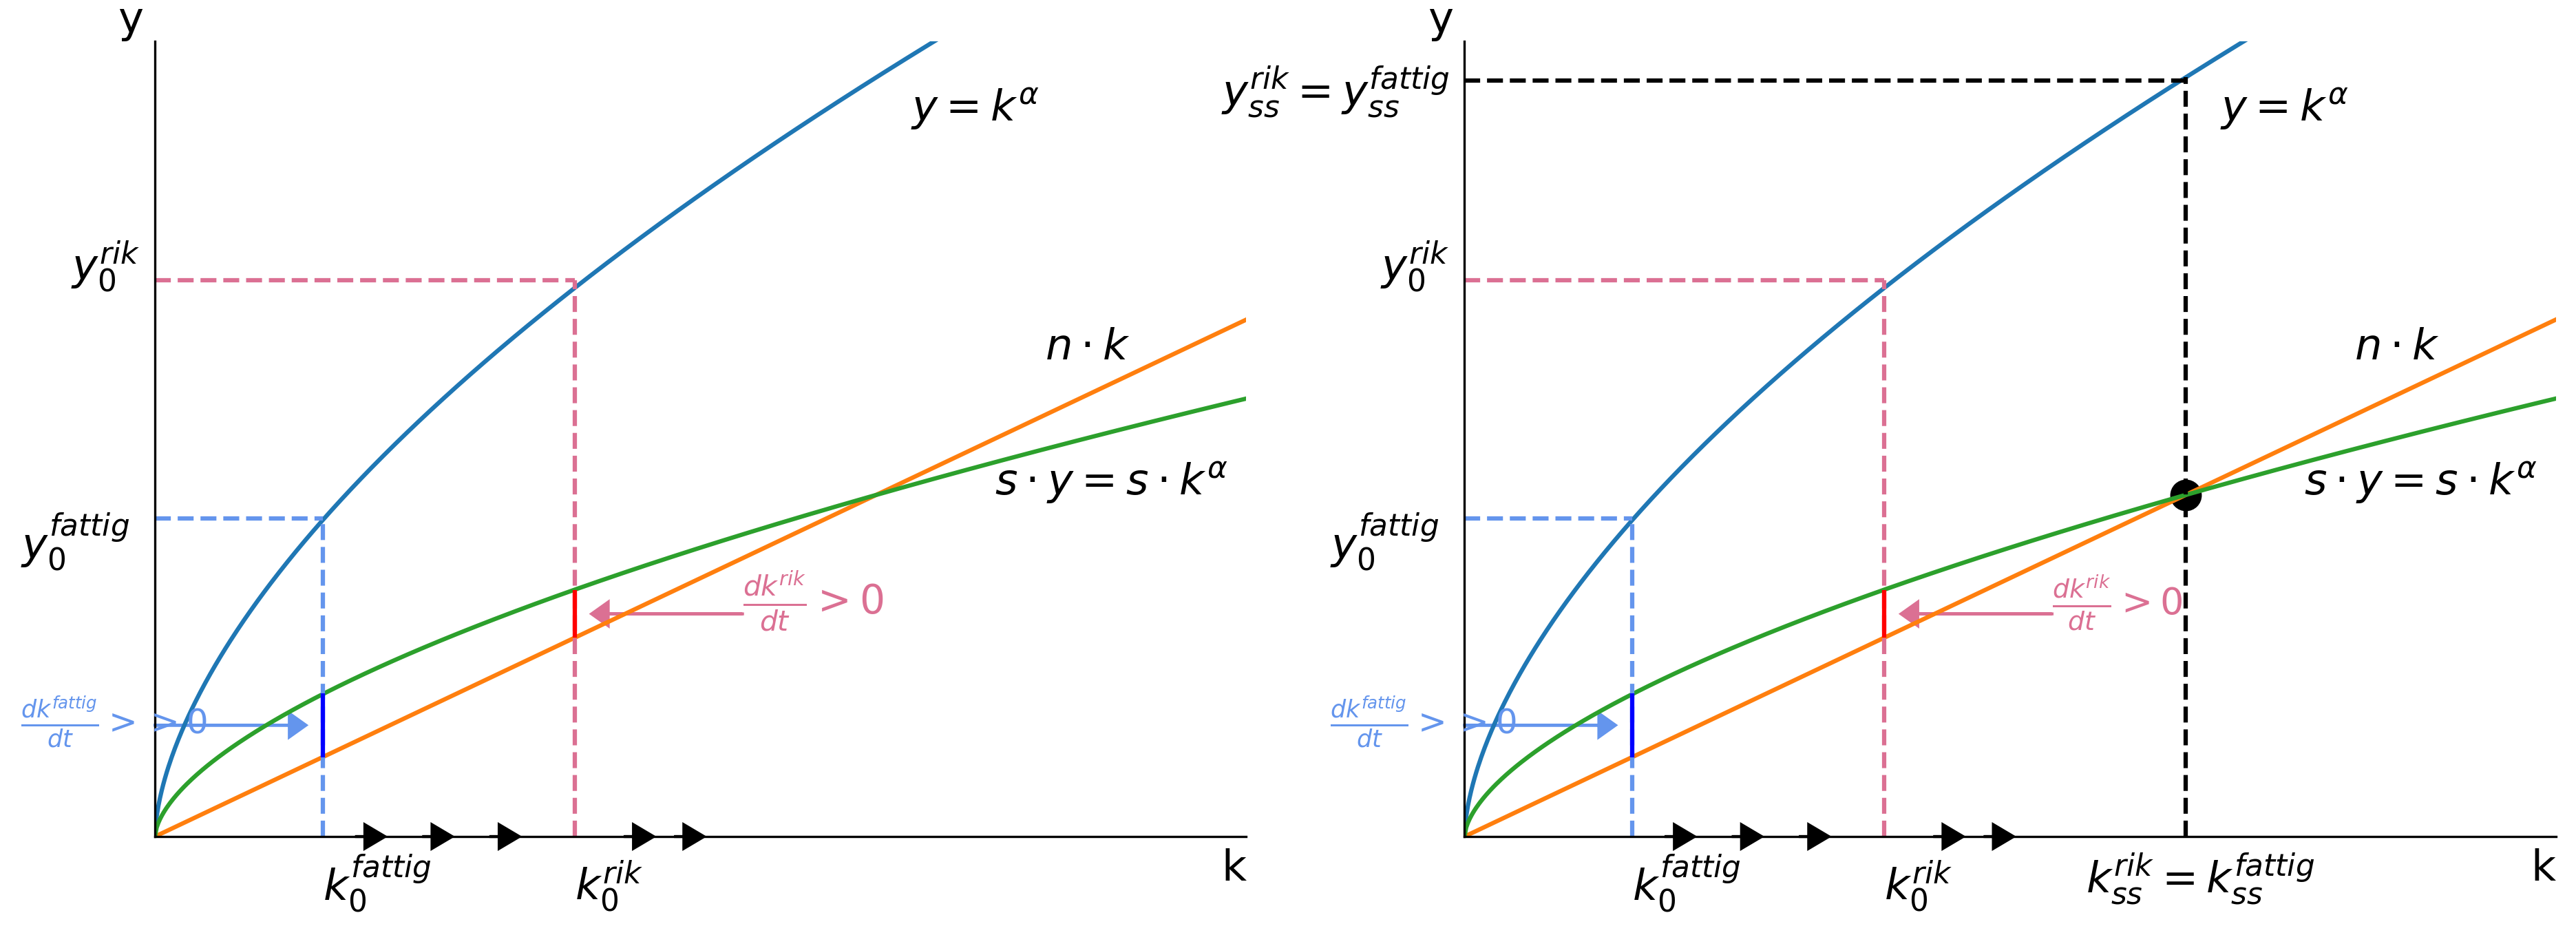
\includegraphics[width=\linewidth]{figurx.png}
  \captionof{figure}{Konvergens i Solow-modellen}
  \label{fig:figurx}
\end{figure}

Dette vil gi det fattige landet en større vekst og begge to vil til
slutt ende med produksjon per arbeider
\(y^{fattig}_{ss} = y^{rik}_{ss}\) og kapital per arbeider
\(k^{fattig}_{ss} = k^{rik}_{ss}\) i steady-state som vises i
likevektspunktet i høyre \autoref{fig:figurx}.

Betingelsesløs konvergens er den minst interessante formen for
konvergens i Solow-modellens predikering av produksjon per arbeider når
man tar hensyn til grunnmodellen siden man kan si det ikke er
realistiske forutsetninger (lukket økonomi) og det da sjeldent vil kunne
relateres til virkeligheten.

\clearpage

\subsection{\texorpdfstring{\textbf{Betinget konvergens} (Ulik nivå på
sparerate og befolkningsvekst, åpen
økonomi)}{Betinget konvergens (Ulik nivå på sparerate og befolkningsvekst, åpen økonomi)}}\label{betinget-konvergens-ulik-nivuxe5-puxe5-sparerate-og-befolkningsvekst-uxe5pen-uxf8konomi}

To land har lik produksjon og åpen økonomi, men med ulik nivå på
sparerate og befolkningsvekst så vil nivå på BNP per arbeider
konvergere, gitt at det er åpne økonomier. Også her starter økonomiene i
forskjellige steady-states, men ender på sikt opp i lik steady-state.

\begin{wrapfigure}{r}{0.5\textwidth}
  \centering
  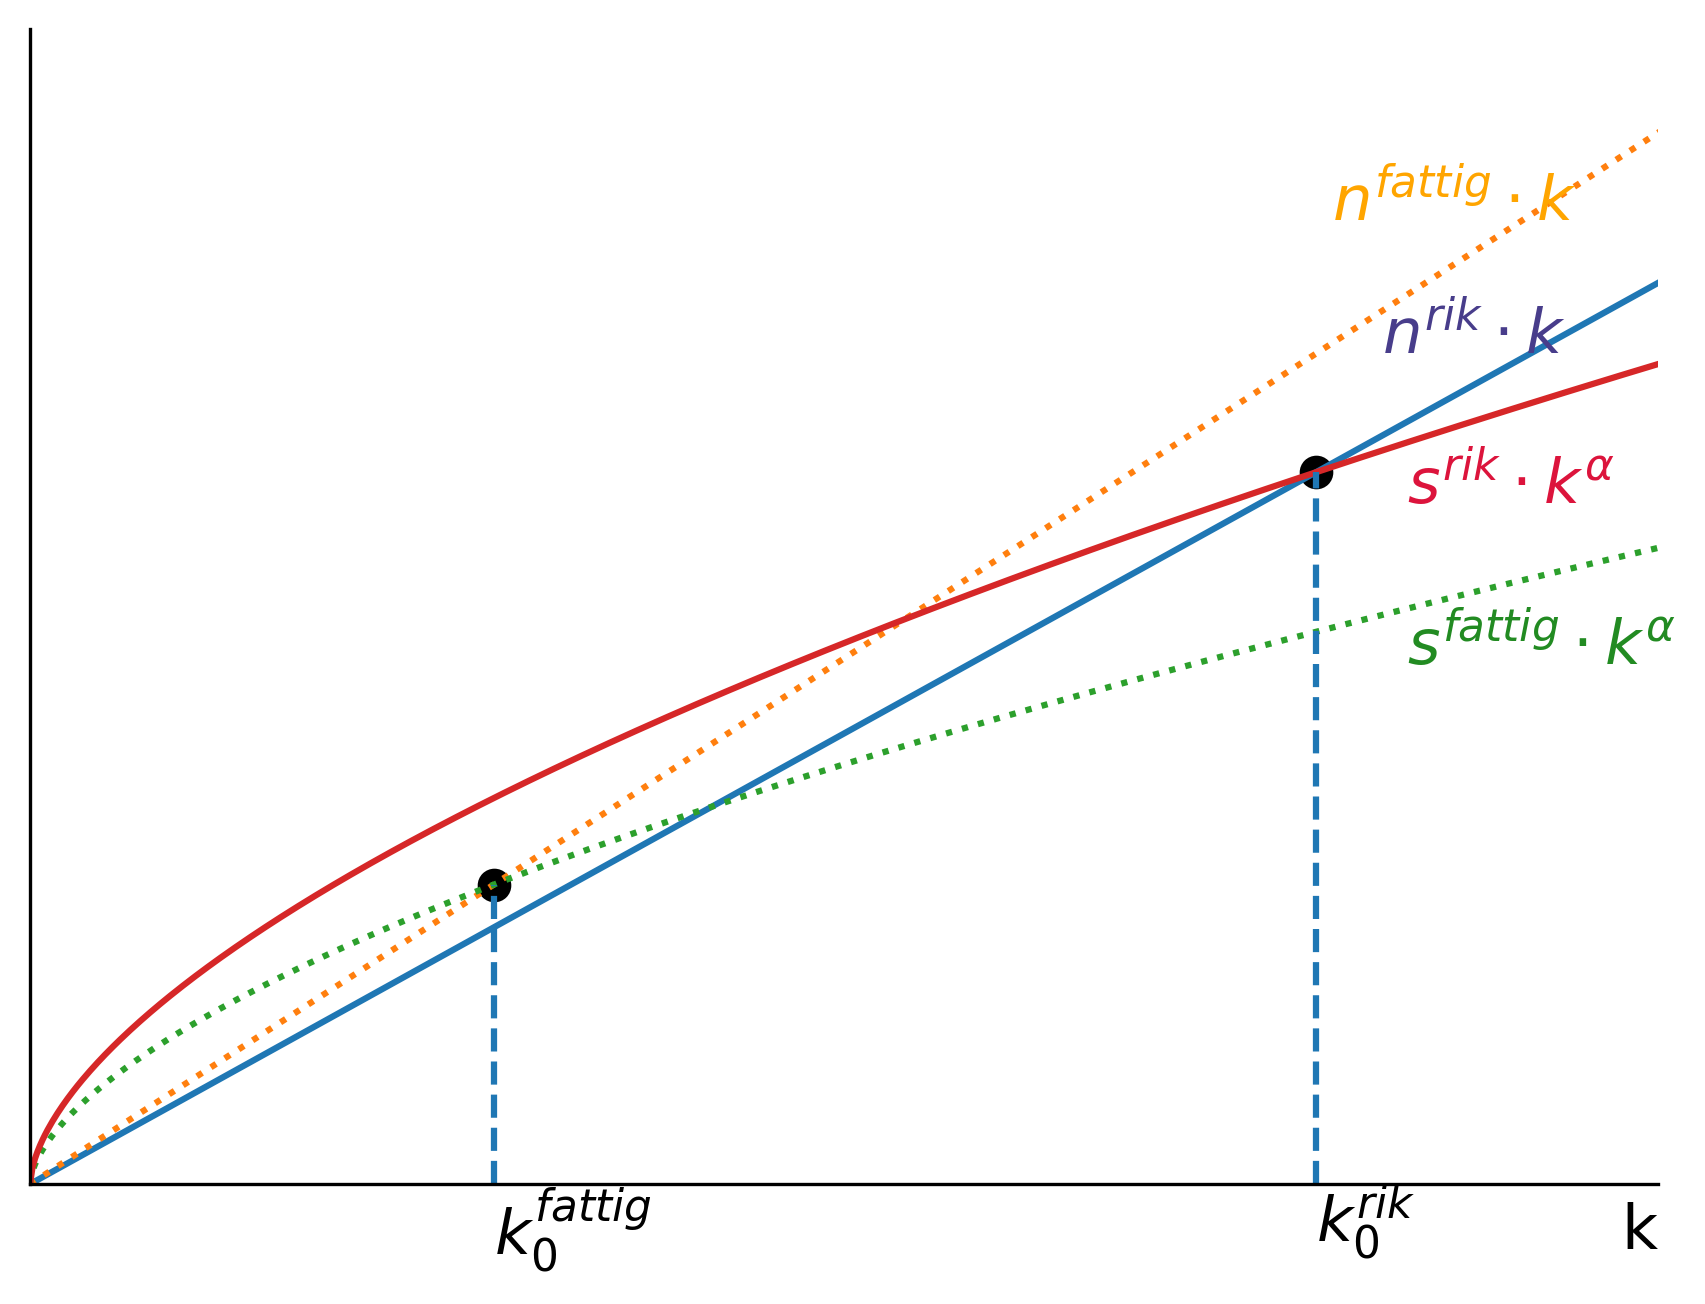
\includegraphics[width=0.5\textwidth]{ubetinget_konvergens.png}
  \captionof{figure}{Betinget konvergens}
  \label{fig:betinget}
  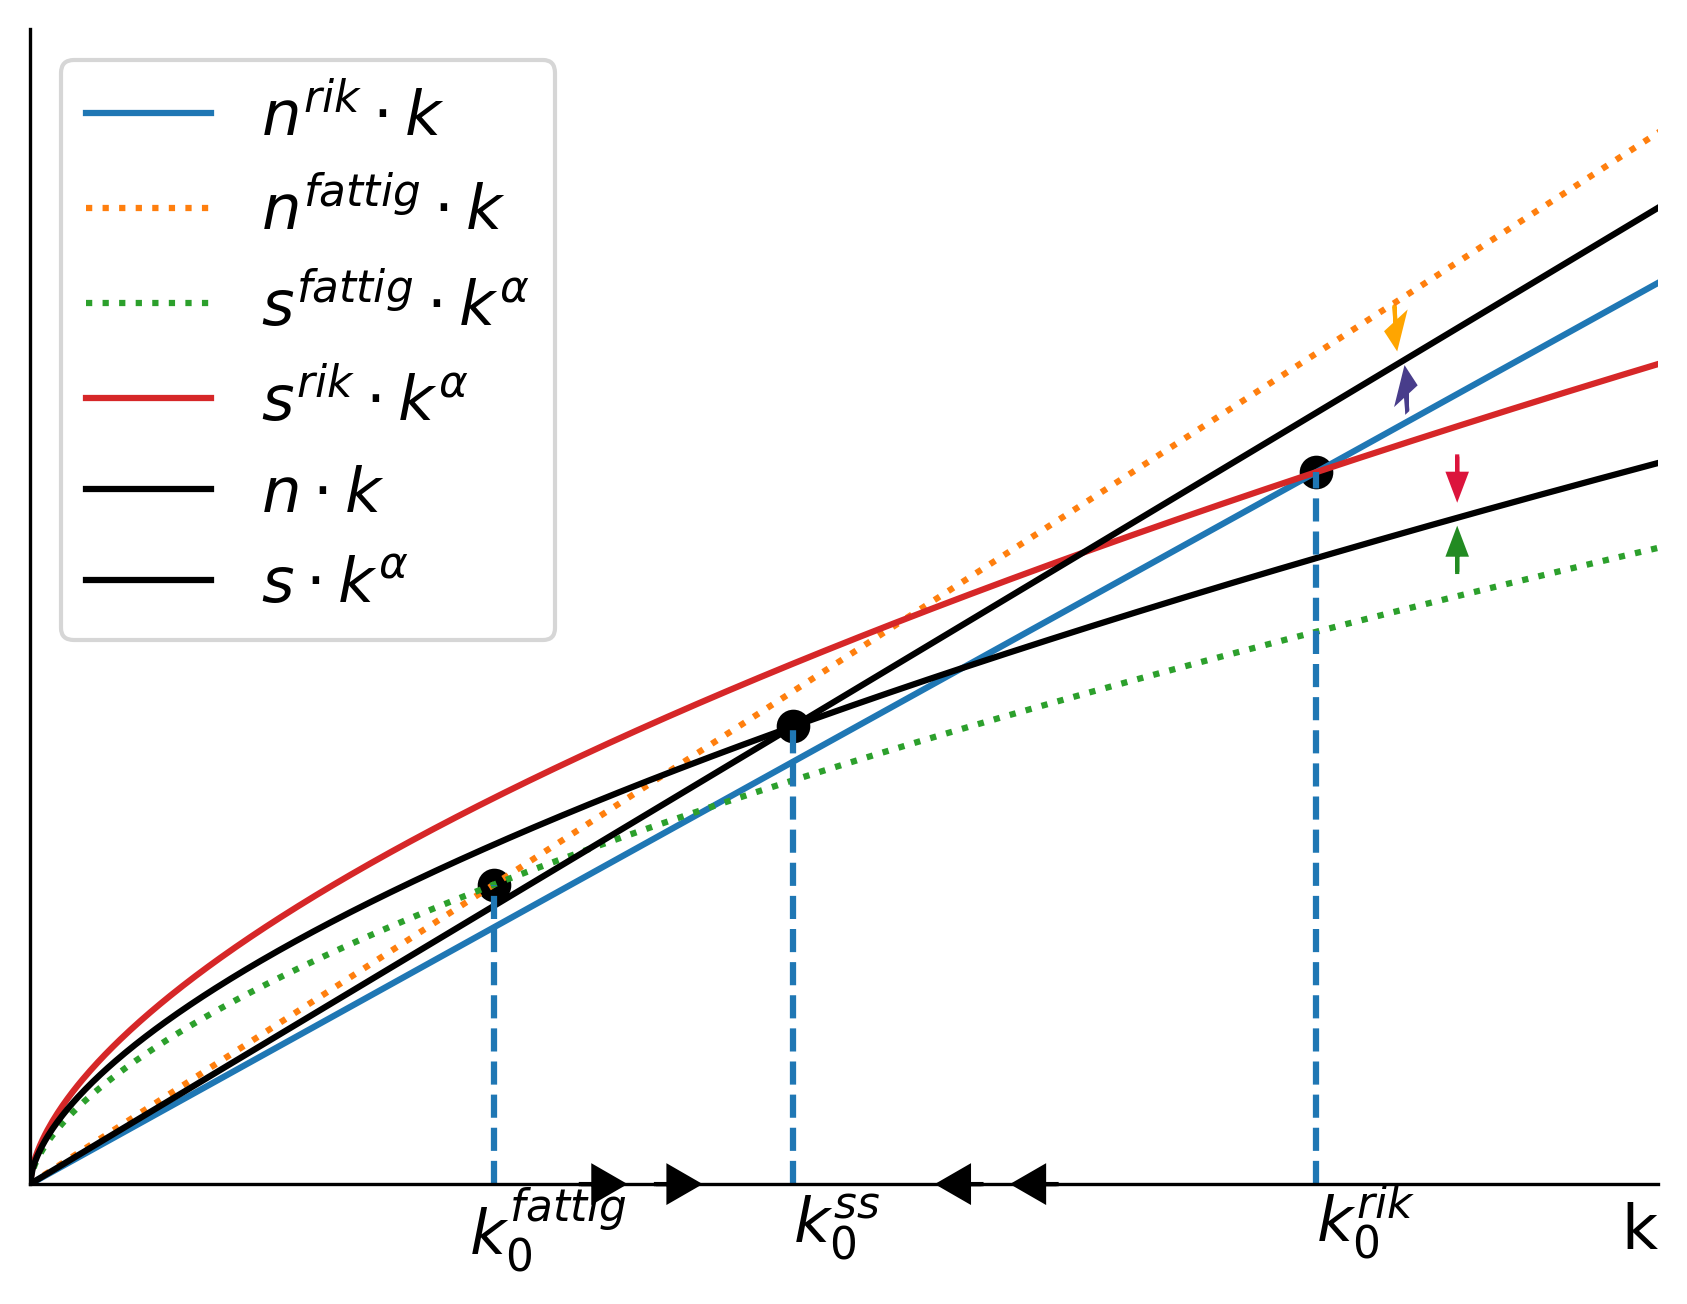
\includegraphics[width=0.5\textwidth]{betinget_konvergens.png}
  \captionof{figure}{Betinget konvergens}
  \label{fig:ubetinget}
  \vspace{-10mm}
\end{wrapfigure}

Det fattige landet vil i starten konvergere i likevektspunktet
\(k_0^{fattig}\) for nødvendige og faktiske investeringer, og det samme
for det rike landet i likevektspunktet for \(k_0^{rik}\). Om det er
lukkede økonomier, vil ikke landene konvergere. Men siden vi har åpen
økonomi så predikerer teorien at siden det fattige landet har lav
sparerate og høy befolkning og det rike landet har høy sparerate men lav
befolkning, så vil arbeidere fra det fattige landet flytte til det rike.
Kapitaleire i det rike landet vil også investere i det fattige landet
siden de vil få bedre avkastning for produksjonsfaktorene der enn
hjemme.

Som man kan se i \autoref{fig:ubetinget} så vil dette føre til at
spareraten i det rike landet presses ned mens spareraten øker i det
fattige landet, og befolkningstallene øker i det rike landet og minker i
det fattige. \(k_0^{rik}\) minker mens \(k_0^{fattig}\) øker og de to
landene vil ende opp i \(k_0^{ss}\) likevekt over tid. Dette er
historisk sett også hva som har skjedd i virkeligheten mellom økonomier,
men trenger ikke alltid være korrekt, siden man i grunnmodellen ikke har
med teknologisk utvikling eller naturressurser som kan predikere at
ulike økonomier kan ende opp i ulike steady-states.

\clearpage

\section{Utfordring 1.3 Solow-modellen med teknologi og
naturressurser}\label{utfordring-1.3-solow-modellen-med-teknologi-og-naturressurser}

Solow-modellen med teknologisk utvikling og naturressurser gir
prediksjoner om hvordan ulike faktorer påvirker vekstraten i BNP per
innbygger på lang sikt.

\subsubsection{Utledning av Solow-modellen med teknologi og
naturressurser (ikke i
steady-state)}\label{utledning-av-solow-modellen-med-teknologi-og-naturressurser-ikke-i-steady-state}

\fbox{
 \addtolength{\linewidth}{-2\fboxsep}%
 \addtolength{\linewidth}{-2\fboxrule}%
\begin{minipage}{\linewidth}
\begin{equation}
    Y(t) = A(K(t)q_k(t))^\alpha(L(t)q_l(t))^\beta (R(t)q_r(t))^\gamma 
\end{equation}
\text{Tar logaritmen av uttrykket:}
\begin{equation}
    log(y(t)) = log(\frac{A_0 K(t) e^{jt})^\alpha (L_0 e^{mt} e^{n t})^{\beta} (R_0 e^{ht} e^{-ut})^\gamma e^{g_At} e^{-n t}}{L_0})
\end{equation}
\text{Deriverer med hensyn på t:}
\begin{equation}
    \frac{\frac{d}{dt} y(t)}{y(t)} = g_A + \gamma h + \alpha j + \beta m + \beta n - n - u \gamma + \alpha \frac{\frac{d}{dt} K(t)}{K(t)}
\end{equation}
\text{Substituerer inn for noen uttrykk som er utledet tidligere:}
\begin{equation*}
    \frac{\partial K}{t} = s\cdot Y \rightarrow \frac{\frac{\partial K}{\partial t}}{K(t)} = \frac{sY}{K} = \left(\frac{sy}{k}\right)
\end{equation*}
\begin{equation*}
    \frac{\frac{d}{dt} y(t)}{y(t)} = g_y
\end{equation*}
\text{Faktoriserer uttrykket så mye som mulig:}
\begin{equation}
    g_y = g_A + \gamma h + \alpha j + \beta m + \beta n - n - u \gamma + \alpha \left(\frac{sy}{k}\right)
\end{equation}
\begin{equation*}
    \theta = g\_A + \gamma h + \alpha j + \beta m 
\end{equation*}
\begin{equation}
    g_y = \theta + \beta n - n - u \gamma + \alpha \left(\frac{sy}{k}\right)
\end{equation}
\begin{equation*}
    \beta+\alpha+\gamma = 1 \rightarrow \beta = \alpha - \gamma +1
\end{equation*}
\begin{equation}
    g_y = \theta + n(-\alpha-\beta+1) - n - u \gamma + \alpha \left(\frac{sy}{k}\right)
\end{equation}
\begin{equation}
    g_y = \theta - \alpha n - n \gamma - u \gamma + \alpha \left(\frac{sy}{k}\right)
\end{equation}
 \end{minipage}
}

\subsubsection{Solow-modellen og faktorer for økonomisk vekst på lang
sikt}\label{solow-modellen-og-faktorer-for-uxf8konomisk-vekst-puxe5-lang-sikt}

Teknologisk fremgang, representert ved en eksogen vekstrate, antas å ha
en positiv, men avtagende, marginal effekt på produksjon per arbeider.

Naturressurser fungerer som en begrensende faktor i modellen. Det er en
begrenset mengde som blir brukt opp.

Uttrykket \(\left(\frac{sy-nk}{k}\right)\) representerer vekstraten i
kapital. Det beregnes ved å multiplisere spareraten med produksjon per
arbeider, og deretter trekke fra produktet av befolkningsvekst-raten og
kapital. Til slutt deles dette med kapital for å få vekstraten i
kapital.

\(\gamma (u+n)\) viser hvor mye naturressurser som brukes opp i forhold
til befolknings-vekstraten. Her representerer \(u\) reduksjonen i
naturressurser, og \(n\) representerer befolkningsveksten.

Ligningen
\(g_y(t) = \theta+ \alpha \frac{sy(t) -nk}{k(t)} - \gamma(u+n)\)
representerer produksjon per arbeider. Vi antar her at teknologien er
konstant.

Hvis \(\theta+ \alpha \frac{sy(t) -nk}{k(t)}\) er mindre enn
\(-\gamma(u+n)\), vil det føre til redusert eller negativ økonomisk
vekst. Dette skjer når naturressurser brukes opp, eller når
befolkningsveksten er høy, noe som fører til at det er flere som skal
dele på kapitalen. Dette reduserer arbeidseffektiviteten, og det er ikke
mulig å investere nok til å opprettholde en stabil tilstand.

Men hvis \(\theta+ \alpha \frac{sy(t) -nk}{k(t)}\) er større enn
\(-\gamma(u+n)\), vil det føre til positiv økonomisk vekst. Dette skjer
når befolkningsveksten er lavere enn investeringskapasiteten, noe som
resulterer i høyere kapital per arbeider. Det kan også skje når
naturressurser ikke brukes overdrevent i produksjonen, eller når sparing
og investering er høy, noe som fører til økt produksjon og økonomisk
vekst.

\clearpage

\section{Referanser}\label{referanser}

\phantomsection\label{refs}
\begin{CSLReferences}{1}{0}
\bibitem[\citeproctext]{ref-hess_2016_economic}
Hess, P. N. (2016). \emph{Economic growth and sustainable development}.
Routledge.

\bibitem[\citeproctext]{ref-Forelesingsnotat}
Mannberg, A. (2023). \emph{SOK-2011 v2024: Utfodring 2}.
\url{https://uit-sok-2011-v2024.github.io/assets/sok2011_utf2_2024.html}

\end{CSLReferences}

\clearpage

\appendix

\section {Appendix Generell KI bruk}

I løpet av koden så kan det ses mange \# kommentarer der det er skrevet
for eks ``\#fillbetween q1 and q2''. Når jeg skriver kode i Visual
Studio Code så har jeg en plugin som heter Github Copilot. Når jeg
skriver slike kommentarer så kan den foresøke å fullføre kodelinjene
mens jeg skriver de. Noen ganger klarer den det, men andre ikke. Det er
vanskelig å dokumentere hvert bruk der den er brukt siden det ``går
veldig fort'' men siden jeg ikke har fått på plass en slik dokumentasjon
så kan all python kode der det er brukt kommentarer antas som at det er
brukt Github Copilot. Nærmere info om dette KI verktøyet kan ses på
\url{https://github.com/features/copilot}

\section {Appendix 1.1 KI bruk}

\section {Appendix Kapittel 1.2 KI bruk}

\section {Appendix Kapittel 1.3 KI bruk}



\end{document}
